% !TEX root = document.tex

\chapter{\label{chap:evaluation}Evaluation}

In this chapter we evaluate the newly introduced SDF3 and Statix specifications for WebDSL. The new specifications have two concrete use-cases, namely serving as a case study for SDF3 and Statix, and being used on a daily basis by WebDSL developers. For both purposes it is useful to gather information about how the specifications behave in various situations. As a result of the case study, we want to show strengths and weaknesses of SDF3 and Statix based on information from the specifications, and for the WebDSL developers we would like to decide whether the new specifications are ready to be used in practice.

For both specifications, we will evaluate their correctness and performance on existing test suites, as well as WebDSL code that is used in practice. Then, we conclude this chapter by discussing the usability of the modernized implementation in practice.

\section{\label{sec:eval-sdf3}Evaluating the WebDSL SDF3 Specification}

  Evaluating the SDF3 specification of the WebDSL grammar is done in two parts: its correctness and its performance in terms of generated parse tables and their run time. In this section we will use the current implementation of the WebDSL grammar in SDF2 as the reference grammar for correctness and performance.

  \subsection{Correctness}

    In this thesis we do not formally prove the correctness of the new grammar. Instead, we parse test suites that are intended for the current SDF2 specification and parse open source WebDSL applications that are used in practice.

    The test suite consists of 231 WebDSL snippets, ranging from single expressions to complete functioning applications. To re-use this test suite for the SDF3 specification, we converted the snippets into SPT tests and the result is that all of the 231 snippets parse succesfully.

    Upon closer inspection of the original test suite, while converting it to an SPT test suite, we concluded it was not a complete test suite of all syntax constructs but mostly contained syntax fragments which were problematic in the past to serve as a regression test suite. For the sake of completion, we decided to extend the SPT test suite, leading to a new total of 1118 SPT tests, where the newly added test have an expected AST result, instead of only expecting the snippets to parse correctly.

    In addition to the test suite, we used two open-source WebDSL applications for verifying that the new parser generated from the SDF3 specification does not suddenly fail or see ambiguities in existing applications:

    \begin{itemize}
      \item \textbf{YellowGrass:} A tag based issue tracker similar to GitHub Issues, complete with access control and used daily by WebDSL developers. YellowGrass consists of 54 WebDSL files plus 20 WebDSL library files and 1 standard library file, coming to a total of 12.898 lines of code spread over 75 files.
      \item \textbf{Reposearch:} A source code search engine that helps to find implementation details, example usages, etc. Reposearch consists of 16 main files, 19 library files and 1 standard library file, totalling at 8.722 lines of code spread over 36 files.
    \end{itemize}

    The result of parsing both applications with the new parser generated with the SDF3 specification is that no ambiguities were found.

    One thing to note in discussing correctness of the WebDSL SDF3 completeness is that, while the results are promising, the SDF3 specification has introduced many new sorts and constructors for disambiguation purposes, and to comply with the Statix Signature Generator expectations. The effect of this change is that the resulting ASTs were not compared and we can therefore not guarantee correctness of the disambiguation, other than the subjective confidence gained from handpicking snippets and comparing the ASTs manually.

  \subsection{Performance}

    The performance of a parser of a programming language is essential due to the rest of the compilation chain depending on its output. A requirement to use the parser generated by the new SDF3 specification in practice, is that its run time should not increase substantially.

    Grammar specifications in SDF2 and SDF3 are not interpreted directly. Both formalisms generate a parse table, which is interpreted by the parser implementation JSGLR. JSGLR is an implementation of SGLR parsing in Java, used within the Spoofax Language Workbench. Because of this architecture, it is insightful to inspect the generated parse tables and highlight the differences, as well as comparing the run times of both parsers on the test suite and existing applications.

    \begin{table}[h]
      \begin{tabular}{ |c||c | c | p{2cm} | c | p{2.2cm}| }
        \hline
        Parse table from & States & Gotos & Max gotos per state & Actions & Max actions per state \\
        \hline\hline
        SDF2 & 10.449 & 179.454 & 510 & 62.127 & 107 \\
        \hline
        SDF3 & 12.866 & 244.688 & 821 & 525.728 & 2.491 \\
        \hline
      \end{tabular}
      \caption{\label{tbl:parse-table-differences}Data about the size of the parse tables generated from the SDF2 and SDF3 grammar specifications.}
    \end{table}

    The parse table generated from the SDF3 specification has more states, gotos and actions than the parse table from the SDF2 specification. Even though the described grammar did not change, it is implemented differently, leading to the increase in parse table size. To see the impact of the larger parse table on the run time, we executed the evaluation on YellowGrass, Reposearch and all files in the analysis test suite, which contains complete WebDSL programs as opposed to the syntax test suite.

    To execute the evaluation, we used a 2019 MacBook Pro running macOS Montery 12.2. The machine has a 2,3 GHz 8-core Intel Core i9 with 64 GB RAM available. The evaluation scripts\footnote{https://github.com/metaborg/jsglr2evaluation} were configured to parse the described files with the SDF2 parse table, as well as the SDF3 parse table using the JSGLR1 parser implementation. Using the Java Microbenchmark Harness\footnote{https://github.com/openjdk/jmh}, we timed the run time of the parsers using 5 warmup iterations and 10 regular iterations.

    \begin{figure}
      \begin{tikzpicture}
 
        \begin{axis} [ybar, axis on top,
            title={Benchmark Results (Analysis test suite)},
            ylabel={Run time (ms)},
            bar width=40,
            xmin=0,
            xmax=3,
            xticklabels={,SDF2,SDF3,},
            nodes near coords,
            ymin=0]
         
          \addplot coordinates {(1,394)};
          \addplot coordinates {(2,450)};
         
        \end{axis}
         
        \end{tikzpicture}
      \caption{\label{fig:syntax-performance-charts}Run time of SDF2 definition vs. SDF3 definition}
    \end{figure}

    \begin{itemize}
      \item[TO-DO:]
      \item Parse analysis test suite files with both SDF2 and SDF3, show difference in timings
      \item Parse YellowGrass and RepoSearch with both SDF2 and SDF3, show difference in timings
    \end{itemize}

  \subsection{Maintainability}

    Two of the goals of introducing SDF3 as successor of SDF2 in the syntax formalism family, were to support more declarative syntax definition and to make the syntax definitions more readable and understandable \autocite{AmorimV20}. \Cref{fig:sdf3-maintainability-1} shows snippets of the SDF2 and SDF3 specifications that define a WebDSL for-loop. The snippets show that the SDF3 syntax is more similar to other grammar formalisms such as EBNF \autocite{BackusBGK0NPRSV63} and for this reason we argue that the WebDSL syntax definition in SDF3 is easier to read and understand than its predecessor in SDF2.

    \begin{figure}
      \begin{subfigure}[b]{1\textwidth}
        \begin{minted}[firstline=3]{\sdftwo}
module WebDSL-UI
  exports
  context-free syntax

    "for" "(" Id ":" Sort "in" Exp OptFilter ")"
      "{" TemplateElement* "}" ForSeparator -> TemplateElement {cons("For")}

    "separated-by" "{" TemplateElement* "}" -> ForSeparator{cons("ForSeparator")}
                                            -> ForSeparator{cons("None")}
        \end{minted}
        \caption{\label{fig:sdf3-maintainability-1-sdf2}}
      \end{subfigure}
      \begin{subfigure}[b]{1\textwidth}
        \begin{minted}[firstline=2]{\sdfthree}
module WebDSL-UI
  context-free sorts

    TemplateElement ForSeparator

  context-free syntax

    TemplateElement.For = <
      for ( <VarId> : <Sort> in <Exp> <OptFilter> ) {
        <TemplateElement*>
      } <ForSeparator>
    >

    ForSeparator.ForSeparator     = <separated-by { <TemplateElement*> }>
    ForSeparator.ForSeparatorNone = <>
        \end{minted}
        \caption{\label{fig:sdf3-maintainability-1-sdf3}}
      \end{subfigure}
      \caption{\label{fig:sdf3-maintainability-1}Defining a WebDSL for-loop in SDF2 and SDF3}
    \end{figure}

    However, being easier to read and understand does not automatically make the new syntax definition easier to maintain. The compliance with the Statix Signature Generator\footnote{https://www.spoofax.dev/howtos/statix/signature-generator/} imposes constraints on the grammar, such as disallowing optional sorts, which in the worst case causes the amount of sorts in the grammar to double as described in \cref{subsubsec:sdf3-optional-sorts}. Additionally, disambiguation without the \texttt{prefer} and \texttt{avoid} keywords, as described in \cref{sec:webdsl-sdf3-disambiguation}, creates the need for even more sorts which artificially complicate the grammar definition.

\section{\label{sec:eval-statix}Statix}

  \begin{itemize}
    \item Defining correctness in absence of a formal specification
    \item How correct is the implementation WebDSL
    \item Explain correctness
    \item Edge cases
  \end{itemize}

  \subsection{Correctness}

    \begin{itemize}
      \item Analysis test suite: expect to pass all
      \item Analyze YellowGrass and Reposearch, expect 0 errors
      \item Explain differences
    \end{itemize}

  \subsection{Performance}

    \begin{itemize}
      \item Analyze analysis test suite files with both Stratego and Statix analysis, show difference in timings
      \item Analyze YellowGrass and Reposearch with both Stratego and Statix analysis, show difference in timings
    \end{itemize}

  \subsection{Usability}

    \begin{itemize}
      \item Lack of user-friendliness of the error messages generated by Statix
      \item Can the WebDSL Statix specification be used as formal specification?
      \item Maintainability of the codebase
    \end{itemize}
